%!TEX root = ../report.tex

\begin{landscape}

\section{Appendix} % (fold)
\label{sec:attachments}


\subsection{Appendix A - Work Scheduling Plan} 

The next Figure presents the Gantt Chart for this project. In Table 6 we have a description of objectives for each task.



\begin{figure}[h!]
\centering
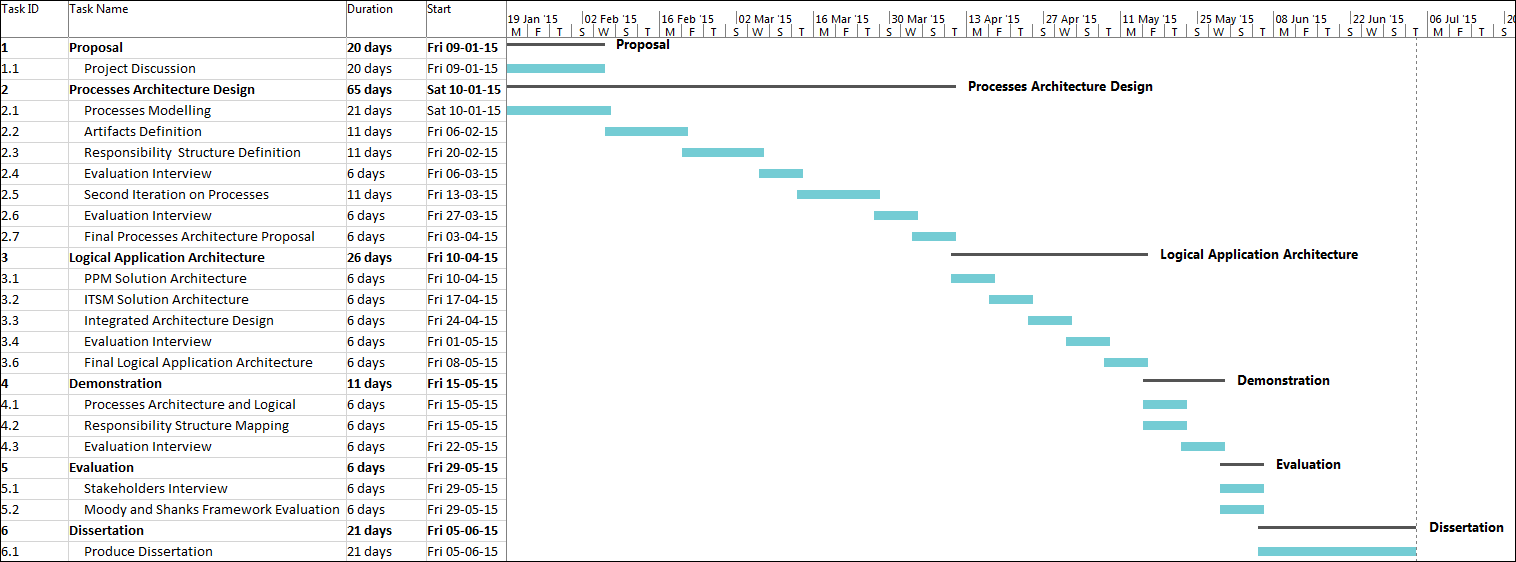
\includegraphics[height=0.55\textheight]{img/GanttChart2.png}
\caption{Gantt Chart for the project.}
\end{figure}

\end{landscape}

\newpage



\begin{table}[h!]
\centering
\resizebox{\textwidth}{!}{%
\begin{tabular}{|l|l|}
\hline
\multicolumn{1}{|c|}{\textbf{Task ID}} & \multicolumn{1}{c|}{\textbf{Objectives}} \\ \hline
\rowcolor[HTML]{68CBD0} 
\textbf{1} & \textbf{Proposal} \\ \hline
1.1 & Prepare project presentation and discussion. \\ \hline
\rowcolor[HTML]{68CBD0} 
\textbf{2} & \textbf{Process Architecture Design} \\ \hline
2.1 & \begin{tabular}[c]{@{}l@{}}Selection of high level processes to include in architecture; \\ Definition of activities for each process; \\ Definition of objectives, inputs and outputs of each activity;\end{tabular} \\ \hline
2.2 & \begin{tabular}[c]{@{}l@{}}Definition of artifacts related to inputs and outputs of each activity; \\ Artifacts design and production;\end{tabular} \\ \hline
2.3 & \begin{tabular}[c]{@{}l@{}}Definition of a responsibility structure to support the processes;\\ Responsibility assignment;\end{tabular} \\ \hline
2.4 & \begin{tabular}[c]{@{}l@{}}Interview with the main stakeholder; \\ Necessary changes definition; \\ Evaluation Report;\end{tabular} \\ \hline
2.5 & \begin{tabular}[c]{@{}l@{}}Iteration on Processes modelling, Artifact definition and \\ responsibility structure definition tasks;\end{tabular} \\ \hline
2.6 & \begin{tabular}[c]{@{}l@{}}Interview with the main stakeholder; \\ Necessary changes definition; \\ Evaluation Report;\end{tabular} \\ \hline
2.7 & \begin{tabular}[c]{@{}l@{}}Iteration on Processes modelling, Artifact definition and responsibilitystructure definition tasks; \\ Final proposal for the Process architecture;\end{tabular} \\ \hline
\rowcolor[HTML]{68CBD0} 
\textbf{3} & \textbf{Logical Application Architecture} \\ \hline
3.1 & \begin{tabular}[c]{@{}l@{}}Definition of PPM solution's features to include into the architecture; \\ Definition of input activities from process architecture to PPM solution; \\ Definition of outputs from PPM Solution;\end{tabular} \\ \hline
3.2 & \begin{tabular}[c]{@{}l@{}}Definition of ITSM solution's features to include into the architecture; \\ Definition of,input activities from process architecture to ITSM solution; \\ Definition of outputs from ITSM Solution;\end{tabular} \\ \hline
3.3 & \begin{tabular}[c]{@{}l@{}}Definition of ITSM and PPM solution's inputs from the processes architecture; \\ Integration with application architectures already present in the organization; \\ Definition of application architecture outputs; \\ Definition of necessary infrastructure;\end{tabular} \\ \hline
3.4 & \begin{tabular}[c]{@{}l@{}}Interview with the main stakeholder; \\ Necessary changes definition; \\ Evaluation Report;\end{tabular} \\ \hline
3.5 & \begin{tabular}[c]{@{}l@{}}Iteration on ITSM and PPM solutions' architecture;\\ Final proposal for the Logical Application architecture;\end{tabular} \\ \hline
\rowcolor[HTML]{68CBD0} 
\textbf{4} & \textbf{Demonstration} \\ \hline
4.1 & \begin{tabular}[c]{@{}l@{}}Process framework and Logical Application Architecture presentation to stakeholders;\\ Process framework application proposal to the organization;\\ Logical application architecture integration on organization proposal;\end{tabular} \\ \hline
4.2 & Mapping between responsibility structure defined and demonstration's organization structure; \\ \hline
4.3 & \begin{tabular}[c]{@{}l@{}}Interview with the main stakeholder; \\ Evaluation Report;\end{tabular} \\ \hline
\rowcolor[HTML]{68CBD0} 
\textbf{5} & \textbf{Evaluation} \\ \hline
5.1 & \begin{tabular}[c]{@{}l@{}}Interview with the main stakeholder; \\ Evaluation Report;\end{tabular} \\ \hline
5.2 & \begin{tabular}[c]{@{}l@{}}Evaluation using Moody and Shanks Framework; \\ Results analysis and reporting;\end{tabular} \\ \hline
\rowcolor[HTML]{68CBD0} 
6 & \textbf{Dissertation} \\ \hline
6.1 & \begin{tabular}[c]{@{}l@{}}Write dissertation;\\ Dissertation presentation;\end{tabular} \\ \hline
\end{tabular}
}
\vspace{2mm}
\caption{Tasks and objectives for the project.}
\label{my-label}
\end{table}

\newpage

\subsection{Appendix B - COBIT 5 Processes by domain} 

The next Figure presents the management and governance processes from COBIT 5 process framework, presented by domain.

\begin{figure}[h!]
\centering
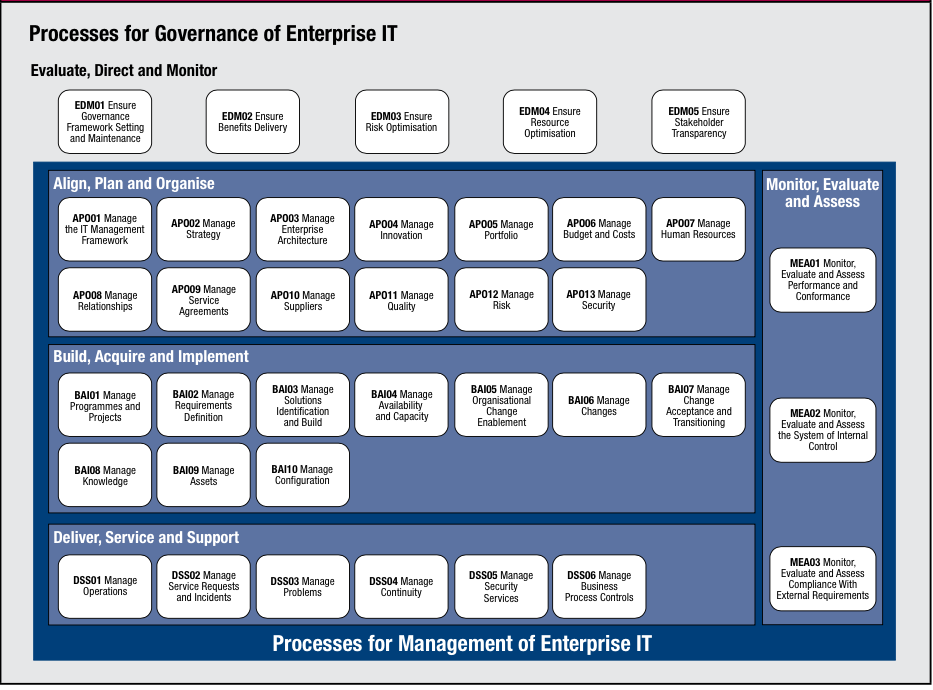
\includegraphics[width=\textwidth]{img/COBIT5ProcessFramework.png}
\caption{COBIT 5 Processes. Extracted from \cite{2012cobit}.}
\end{figure}

\newpage

\subsection{Appendix C - ISO 19011 Audit Programme Management process} 

The next figure presents the process flow purposed by ISO 19011 International standard for Audit programmes management.

\begin{figure}[h!]
\centering
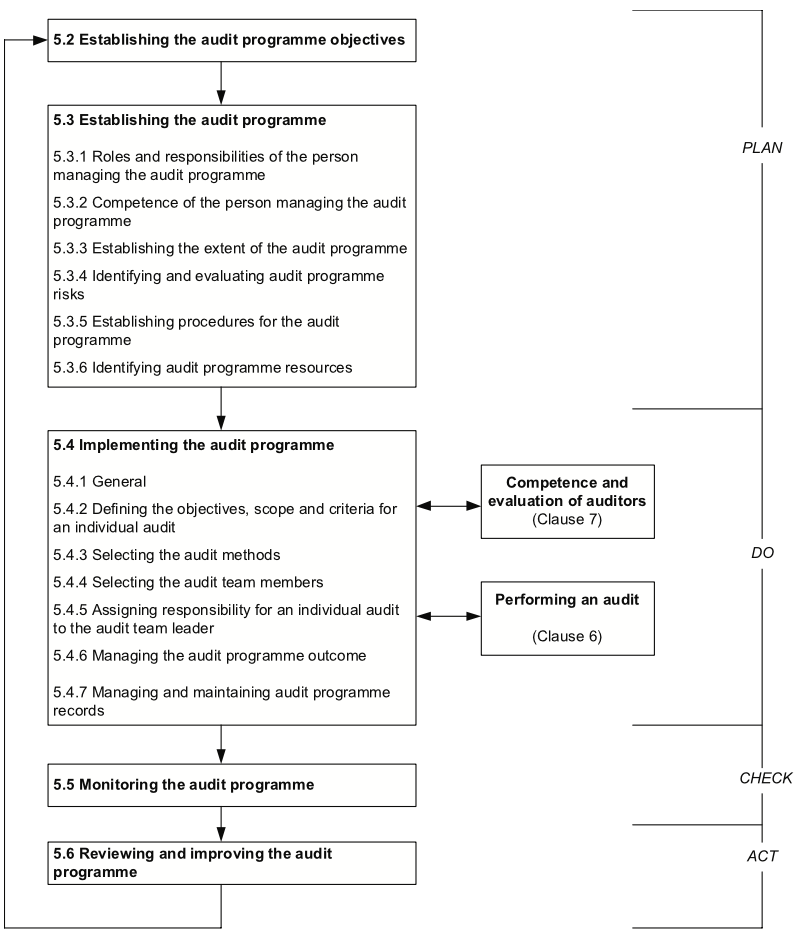
\includegraphics[width=0.9\textwidth]{img/ISO19011AuditProcess.png}
\caption{ISO 19011 Audit Programme Management process. Extracted from \cite{ISO19011}.}
\end{figure}




